% Build: xelatex paper.tex (run twice). Figures: see make_figures.py.
% Numbers: tables come from results/*.json; everything else from
% scripts/paper_stats.py, which writes results/paper_stats.json.
\documentclass[11pt,a4paper]{article}

\usepackage{fontspec}
\usepackage[margin=1in]{geometry}
\usepackage{amsmath}
\usepackage{booktabs}
\usepackage{graphicx}
\usepackage{caption}
\usepackage{float}
\usepackage{xcolor}
\usepackage{tikz}
\usetikzlibrary{shapes.geometric,arrows.meta,positioning}
\usepackage[colorlinks=true,linkcolor=black,citecolor=black,urlcolor=blue!50!black]{hyperref}

\setmainfont{Times New Roman}
\setsansfont{Helvetica}
\setmonofont[Scale=0.9]{Menlo}

\TeXXeTstate=1
\newfontfamily\arabicfont[Script=Arabic,Scale=1.05]{Geeza Pro}
\newcommand{\ar}[1]{{\beginR\arabicfont #1\endR}}

\captionsetup{font=small,labelfont=bf}
\setlength{\parskip}{0.45em}
\setlength{\parindent}{0pt}
\frenchspacing

\title{\textbf{Confidence-routed arbitration between a vision-language model
and a classical OCR engine for Arabic word recognition}}
\author{Mohamed ElhajSuliman Elnaim Suliman\\[0.3em]
\small Code and run files: \url{https://github.com/moelhaj996/mo-ocr-v3}}
\date{September 2026}

\begin{document}
\maketitle

\begin{abstract}
\noindent
On 1,750 held-out images of printed Arabic words, Qwen2-VL-2B, a small
vision-language model, is exactly right on 29.4\% of words, about twice the
rate of EasyOCR (14.1\%). It misreads another 49\% in ordinary ways, and on
22\% it produces long off-topic text, mostly refusals and echoes of the
prompt. That last group drives its corpus character error rate to 2.35. This
report describes MO-OCR, which chooses between the two engines using only the
language model's own output. A length and script check removes most of the
off-topic text, and a threshold on the geometric mean of the token
probabilities sends low-confidence readings to EasyOCR. Neither test is
enough alone. The rule was designed on 250 images kept apart from the held-out
split. On the held-out split it lowers the character error rate from 0.2294 to
0.1710, a difference of −0.0584 (95\% paired bootstrap interval −0.0664 to
−0.0505), and raises exact match to 32.7\%. The result is sensitive to one
limit in the length check: with the limit I first used, the error rate is
0.2057, and fifteen outputs account for the difference. Two ideas that I
expected to help did not. Three community
Arabic TrOCR checkpoints had character error rates between 0.71 and 0.89 on a
ten-image screen and a fourth failed to run. Reranking with a masked language
model never fixed more words than it broke.
The evaluation covers low-resolution printed single words from one source
whose provenance I could not fully establish (Section~\ref{sec:data}). Code
and run files are public.
\end{abstract}

\section{Introduction}

A vision-language model with two billion parameters now runs on a laptop and
can read text in an image. I wanted to know whether such a model could replace
a classical OCR engine for Arabic, or at least improve one. It cannot replace
one, but it can improve one if its bad outputs are filtered out.

Qwen2-VL-2B \cite{qwen2vl} often reads a printed Arabic word perfectly. On the
held-out data used here it gets 515 of 1,750 words exactly right, against 246
for EasyOCR \cite{easyocr}. But on 385 words it does not transcribe anything.
Mostly it apologizes or repeats the instruction back, and these outputs run to
a median of 87 characters where the reference word averages under eight.
Character error rate punishes that heavily, so the model with the best exact
match also has by far the worst error rate.

EasyOCR fails in a different way. It never produced an output with a character
error rate above 1 on this data. Its mistakes are small, and the most common
are single letters that differ from the correct one only in their dots, such
as \ar{ي} read as \ar{ب} or \ar{ت} read as \ar{ن}.

When two systems fail differently it makes sense to combine them, an idea at
least as old as ROVER, which did it for speech recognizers in 1997
\cite{rover}. The question I ask here is narrower and empirical: can the
language model's bad outputs be recognized cheaply, without ground truth, well
enough that routing between the two engines beats both? On this data the
answer is yes.

I give a routing rule with two tests and measure its effect on a held-out
split. An ablation shows what each test contributes and how much the result
depends on one hand-set limit. An error analysis explains where the gain comes
from: the engines disagree on 1,620 of 1,750 words, and a perfect router would
reach a character error rate of 0.1449. I also report two negative results,
and I describe the evaluation harness together with what two rounds of review
found in it, because several of the defects were of a kind that silently
changes reported numbers.

The scope is narrow. Everything is measured on 2,000 low-resolution printed
word images from a single source, with one model checkpoint per engine and one
prompt, on one machine.

\section{Related work}

EasyOCR pairs the CRAFT text detector \cite{craft} with a convolutional
recurrent recognizer trained with a CTC loss \cite{crnn}. TrOCR \cite{trocr}
replaced that design with an image transformer encoder and a text transformer
decoder. Its authors released no Arabic checkpoint, so Arabic use depends on
community fine-tunes. General vision-language models such as Qwen2-VL
\cite{qwen2vl} are not dedicated OCR engines, although reading text in images
is among the tasks they are trained for.

Combining recognizers goes back at least to ROVER \cite{rover}, which aligns the
outputs of several speech recognizers and votes. The arbitration used here is
simpler. It picks one engine's whole output per image instead of voting inside
the string, which suits the case where one engine's failures are total.

For post-correction I tested masked language model scoring \cite{mlmscoring}
with CAMeLBERT \cite{camelbert}, an Arabic BERT model. For document structure
I integrated LayoutLMv3 \cite{layoutlmv3} but could not evaluate it.

The standard Arabic benchmarks are APTI \cite{apti} for printed text and KHATT
\cite{khatt} for handwriting. Both are distributed under a registration form,
and I did not use either. Significance testing follows the bootstrap
\cite{efron} in the paired form that Koehn described for comparing translation
systems \cite{koehn}.

\section{System}

\subsection{Recognizers}

The classical engine is EasyOCR 1.7.2 with its Arabic model, run on CPU with
its default text detector. When the detector returns several regions I join
them in right-to-left reading order.

The vision-language engine is Qwen2-VL-2B-Instruct in half precision on Apple's
Metal backend. It receives the image with a one-sentence Arabic instruction to
copy the text exactly and add nothing, and it decodes greedily for at most 64
new tokens. The processor resizes each image to between 64 and 640 visual
patches of 28 by 28 pixels. I used the checkpoint as cached in May 2026 and
did not pin a revision. The model's confidence is the exponential of the mean
log probability of the generated tokens, that is, the geometric mean of their
probabilities.

\subsection{How the vision-language model fails}

Figure~\ref{fig:outcomes} shows the split. EasyOCR is wrong on most words but
never badly wrong. Qwen2-VL is exactly right more than twice as often and
badly wrong on more than one word in five.

\begin{figure}[!htb]
\centering
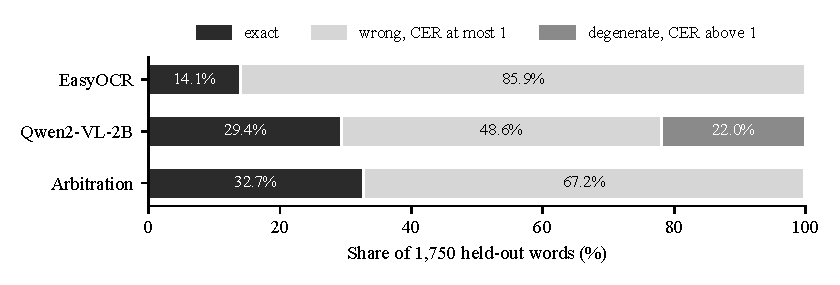
\includegraphics[width=0.92\linewidth]{figures/outcomes.pdf}
\caption{Outcome of each system on the 1,750 held-out words, after scoring
normalization. A degenerate output is one whose character error rate exceeds 1,
which requires the output to be longer than the reference.}
\label{fig:outcomes}
\end{figure}

I sorted the 385 degenerate outputs by simple text rules. The largest group,
229, are refusals in Arabic along the lines of ``I am sorry, but I cannot
understand Arabic''. Oddly, 225 of those open with two Japanese characters
before switching to Arabic. Another 73 repeat or paraphrase the instruction,
and 19 are in Latin script. The remaining 64 are a mixture that includes
general remarks about Arabic script and stock phrases. Most of these outputs
can be caught without a reference, because 359 are longer than 30 characters
and 244 contain letters that are not Arabic.

\subsection{Arbitration}
\label{sec:arbitration}

The router reads the image with Qwen2-VL first and keeps that text unless one
of two tests fails (Figure~\ref{fig:pipeline}).

The first test is a degeneration flag. An output is flagged if it is longer
than 30 characters or contains at least two letters outside the Arabic Unicode
block. On the held-out split the flag fired on 401 outputs. It caught 369 of
the 385 degenerate ones and did not fire on any of the 515 exact ones.

The second test is a confidence threshold. If the confidence defined above is
below 0.40 the output is rejected. This catches most degenerate outputs that
slip past the flag, and it also rejects many ordinary misreadings, which
turns out to matter more (Section~\ref{sec:ablation}).

A rejected image is read by EasyOCR instead. EasyOCR's own confidence is not
used.

\begin{figure}[!htb]
\centering
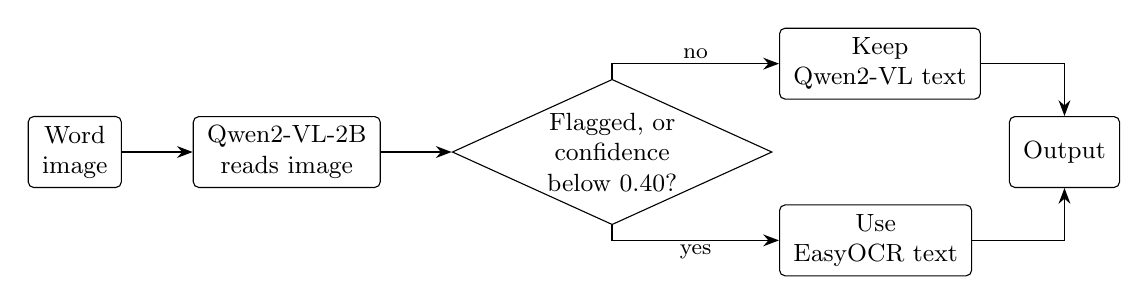
\begin{tikzpicture}[
  node distance=7mm and 9mm,
  box/.style={draw, rounded corners=2pt, align=center, font=\small,
              minimum height=9mm, inner xsep=5pt},
  gate/.style={draw, diamond, aspect=2.2, align=center, font=\small,
               inner sep=1pt},
  arr/.style={-{Stealth[length=2mm]}, semithick},
  lab/.style={font=\footnotesize, inner sep=1.5pt}
]
\node[box] (img) {Word\\image};
\node[box, right=of img] (qwen) {Qwen2-VL-2B\\reads image};
\node[gate, right=of qwen] (gate) {Flagged, or\\confidence\\below 0.40?};
\node[box, above right=2mm and 11mm of gate] (keep) {Keep\\Qwen2-VL text};
\node[box, below right=2mm and 11mm of gate] (fall) {Use\\EasyOCR text};
\node[box, right=30mm of gate] (out) {Output};
\draw[arr] (img) -- (qwen);
\draw[arr] (qwen) -- (gate);
\draw[arr] (gate.north) |- node[lab, above, pos=0.75] {no} (keep.west);
\draw[arr] (gate.south) |- node[lab, below, pos=0.75] {yes} (fall.west);
\draw[arr] (keep.east) -| (out.north);
\draw[arr] (fall.east) -| (out.south);
\end{tikzpicture}
\caption{The arbitration rule. Both tests use only the model's own output.}
\label{fig:pipeline}
\end{figure}

How the rule was arrived at matters for reading the results, so here is the
order of events. I designed it on a pilot set of 50 images, the first data
either engine read. On those 50 images Qwen2-VL's confidence correlated with
exact correctness at \emph{r} = 0.48 and EasyOCR's at \emph{r} = 0.09, which is why
Qwen2-VL is the primary engine and EasyOCR's confidence is ignored. The first
flag, with limits of 40 characters and three non-Arabic letters, was also
written from those outputs. I then tuned the confidence threshold on a
separate development split of 200 images (Section~\ref{sec:threshold}).

After that I looked at the pilot set again and saw two refusals pass both
tests, each just under both flag limits, so I lowered the limits to 30 and
two. On the development split this changed no output, because the confidence
threshold already rejected every output the tighter flag adds. The held-out
split had not been scored. When it was, the change turned out to matter a
great deal, and Section~\ref{sec:ablation} gives the result under both
versions of the flag.

\subsection{Pages and visual order}

Feeding a whole multi-line page to Qwen2-VL exposed a separate problem. The
model returned each line reversed character by character, in the order the
glyphs appear on screen from left to right, and without line breaks. A string
like that scores as almost entirely wrong although the model has read every
letter.

The repository contains a repair for this. It compares an output with its
reversal using orthographic facts that reversal destroys, for instance that
the article \ar{ال} begins words and that \ar{ة} ends them, and it flips the
text only when the evidence is clear. Replaying the repair over all 2,000
stored word outputs changed none of them, so it has no effect on the numbers
in this report. A page mode also exists. It segments the page with the EasyOCR
detector and applies a stricter variant of the rule to each region, with a
confidence bar of 0.70 for regions of line length. I tried it on one
screenshot of dialectal poetry, and I set that bar by eye on the same
screenshot. It produced the correct words in the correct order. One image is
an anecdote, and I make no accuracy claim for pages.

\section{Evaluation protocol}

\subsection{Data}
\label{sec:data}

The data is 2,000 grayscale images of single printed Arabic words, each 35
pixels high and between 45 and 113 pixels wide, with a text file holding the
word. The held-out references are 7 to 10 characters long. There are no
digits and no multi-word items.

The provenance of this data is weaker than I would like. The images are the
first 2,000 rows of the training split of a Hugging Face dataset,
\texttt{mssqpi/Arabic-OCR-Dataset}, downloaded in May 2026 by a script from an
earlier version of this project. That script saved them in a folder called
\texttt{apti}, and the name spread into the manifest, the result files and,
until this report was written, the repository's documentation. I have no
evidence that the images come from the APTI database \cite{apti}, and I do not
claim that they do. On 30 September 2026 the Hugging Face dataset returned an
access error, so it had been removed or made private, and I could not read its
card or confirm its license. Two projects that used it while it was public
describe it as about 2.16 million image and text pairs with labels of at most
10 characters, which is consistent with what I
have.\footnote{\url{https://huggingface.co/Ali0044/Qalam-Net} and
\url{https://github.com/IsmaelMousa/arabic-image-to-text}, both read on 30
September 2026.} The images look synthetic: clean renderings with no scanning
noise.

This has two consequences. The results describe this particular set of small
synthetic renderings and nothing broader. And a reader cannot currently obtain
the images from the original source, which limits reproduction to rescoring
the published run files. The manifest records a SHA-256 hash for each image
and text file.

The 2,000 items were shuffled once with a fixed seed and divided into a pilot
set of 50, a development split of 200, and a held-out split of 1,750. (The
repository calls the pilot set ``golden''.) The design of the rule and the flag
limits come from the pilot set, and the confidence threshold from the
development split. No decision used the held-out split, which was scored once
with the final rule. The additional held-out figures in
Section~\ref{sec:ablation} were computed afterwards and are marked as such.

\subsection{Normalization}

Arabic admits several spellings that a reader treats as the same word. I
score every run twice, on raw Unicode and on normalized text, and report both.

Scoring normalization removes invisible characters and tatweel, applies
Unicode compatibility normalization (NFKC) \cite{uax15}, strips diacritics,
folds the hamza, madda and wasla forms of alef to bare alef, maps \ar{ة} to
\ar{ه} and \ar{ى} to \ar{ي}, converts Arabic-Indic digits to ASCII, collapses
whitespace, and ends with a canonical composition pass (NFC). It is applied
to reference and hypothesis alike. Habash describes these foldings for Modern
Standard Arabic \cite{habash}. The alef and \ar{ى} foldings are near
universal and the \ar{ة} folding is less common. All of them would be wrong
for dialectal text, where some of the merged forms carry meaning. The text the
system outputs is not normalized in this way. It keeps its diacritics and
hamzas.

\subsection{Metrics and statistics}

Character error rate is Levenshtein distance \cite{levenshtein} divided by
reference length. The primary figure is the corpus rate, total edits over
total reference characters. Exact match is the share of words with zero
edits after normalization. I do not report word error rate. Every reference is
a single word, so it would restate exact match.

Comparisons between systems use a paired bootstrap with 10,000 resamples of
the words \cite{efron,koehn}. The same resampled indices are applied to both
systems, and the interval is on the difference.

A recognizer that raises an exception is scored as a complete miss and also
counted separately.

The arbitration results are computed by replaying the routing rule over the
stored outputs of the two engines. Routing depends only on the stored text and
confidence, so the replay is exact, but the combined system was not run end to
end on the full split.

\subsection{Auditing the harness}
\label{sec:audit}

Before computing final numbers I had the harness reviewed adversarially. I
gave each of several sessions of an AI assistant one lens, such as statistics
or Unicode handling, and asked it to find defects that would change a reported
number. Each claim then went to a second session whose job was to refute it
by reproduction. Fourteen claims went in and twelve survived.

Some were serious. Compatibility normalization ran before invisible characters
were stripped, so two strings that differed only by an invisible joiner
normalized to different results, and normalizing a string twice could give a
different answer from normalizing it once. The corpus error rate added a
phantom character to the denominator for every empty reference. The script
that compares two runs never checked that they shared the same ground truth.

I fixed all twelve, added eight regression tests, and rescored the stored
predictions. No reported number changed at four decimal places, but only
because this dataset has no empty references and no stray joiners. On data
that has them the same defects would have changed the numbers.

A second review of the same kind, run on a draft of this report, found more.
The flag-only figures in the draft had been computed with the older flag. The
draft understated how much the flag change affects the held-out result. And
the language model corrector of Section~\ref{sec:rerank} had a defect in its
candidate generator. All three are corrected here, and the corrector
experiment was rerun.

The raw output of one check is easy to misread. The harness counts words
whose reversed hypothesis scores better than the hypothesis itself, as a
guard against text stored in visual order. For Qwen2-VL on the held-out split
that count is 109. None of these is a real reversal. In 101 cases the output
is degenerate, and reversing a long wrong string sometimes lowers its edit
distance by an edit or two. In no case did reversal bring the error rate to
0.2 or below. The check would be more useful if it counted only reversals
that produce a near-correct word.

\section{Results}

\subsection{Held-out results}

\begin{table}[H]
\centering
\small
\begin{tabular}{lccccc}
\toprule
 & \multicolumn{3}{c}{CER, normalized} & \multicolumn{2}{c}{Held-out only} \\
\cmidrule(lr){2-4}\cmidrule(lr){5-6}
System & Pilot & Dev & Held-out & CER raw & Exact match \\
 & \emph{n} = 50 & \emph{n} = 200 & \emph{n} = 1750 & & \\
\midrule
EasyOCR & 0.2332 & 0.2332 & 0.2294 & 0.2538 & 14.1\% \\
Qwen2-VL-2B & 2.6321 & 2.7466 & 2.3470 & 2.3729 & 29.4\% \\
Arbitration & 0.1684 & 0.1666 & \textbf{0.1710} & 0.1867 & \textbf{32.7\%} \\
\bottomrule
\end{tabular}
\caption{Corpus character error rate and exact match. The pilot and
development figures for arbitration are in-sample, since the rule was designed
and tuned on those images. No run had a failure.}
\label{tab:main}
\end{table}

Arbitration lowers the held-out error rate from 0.2294 to 0.1710
(Table~\ref{tab:main}). The difference is −0.0584 with a 95\% interval of
−0.0664 to −0.0505, and none of the 10,000 resamples produced a difference
of zero or more. In relative terms the error rate falls by 25\%. Exact match
rises from 246 words to 572. On raw text the difference is −0.0671, with an
interval of −0.0756 to −0.0588.

Of the 1,750 words, 851 were routed to EasyOCR and 899 kept the Qwen2-VL
text. Two degenerate outputs survived both tests. The threshold also threw
away 38 readings that were exactly right.

The gain holds across word lengths (Table~\ref{tab:slices}). The improvement
in exact match on long words is large because EasyOCR rarely gets a word of
nine or ten letters entirely right.

\begin{table}[H]
\centering
\small
\begin{tabular}{lrcccc}
\toprule
 & & \multicolumn{2}{c}{EasyOCR} & \multicolumn{2}{c}{Arbitration} \\
\cmidrule(lr){3-4}\cmidrule(lr){5-6}
Reference length & \emph{n} & CER & Exact & CER & Exact \\
\midrule
7 or 8 characters & 1408 & 0.2219 & 16.6\% & 0.1703 & 34.5\% \\
9 or 10 characters & 342 & 0.2536 & 3.5\% & 0.1734 & 25.1\% \\
\bottomrule
\end{tabular}
\caption{Held-out results by length of the raw reference. Error rates are on
normalized text.}
\label{tab:slices}
\end{table}

\subsection{Choosing the threshold}
\label{sec:threshold}

Figure~\ref{fig:sweep} shows the development split. The error rate is lowest
at a threshold of 0.35 and stays within 0.01 of that from 0.30 to 0.45. It
rises clearly from 0.50. Thresholds below 0.30 were not tried. I chose 0.40,
inside that range and one step above the minimum, because with 200 images the
differences among 0.30 to 0.45 are noise.

The flag alone brings the development error rate from 0.2332 to 0.1992. The
interval on that difference, −0.0654 to −0.0007, only just excludes zero.

\begin{figure}[!htb]
\centering
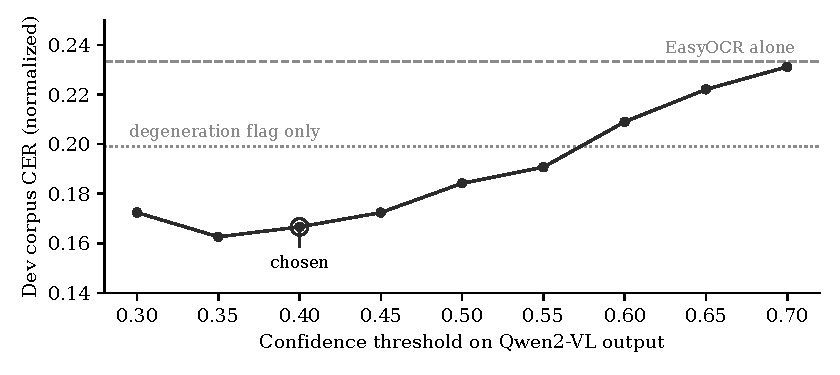
\includegraphics[width=0.92\linewidth]{figures/sweep.pdf}
\caption{Development split error rate as a function of the confidence
threshold. Outputs below the threshold are replaced by the EasyOCR reading.}
\label{fig:sweep}
\end{figure}

\subsection{What each test contributes}
\label{sec:ablation}

Table~\ref{tab:ablation} replays several rules over the held-out outputs. I
computed these after the main result, to understand it. None was used to
choose anything.

\begin{table}[H]
\centering
\small
\begin{tabular}{lccc}
\toprule
Rule & CER & Difference & 95\% interval \\
\midrule
EasyOCR alone & 0.2294 & & \\
Flag only & 0.2235 & −0.0059 & −0.0195 to +0.0079 \\
Confidence threshold only & 0.8415 & +0.6122 & +0.4886 to +0.7446 \\
Original flag and threshold & 0.2057 & −0.0236 & −0.0424 to −0.0035 \\
Flag and threshold (reported) & 0.1710 & −0.0584 & −0.0664 to −0.0505 \\
\midrule
Perfect degenerate detector & 0.2158 & −0.0136 & −0.0250 to −0.0023 \\
Perfect router & 0.1449 & −0.0845 & −0.0909 to −0.0783 \\
\bottomrule
\end{tabular}
\caption{Held-out error rate under different routing rules, with the
difference from EasyOCR alone. The last two rows use the reference and are
bounds, not systems.}
\label{tab:ablation}
\end{table}

Removing degenerate output is not where most of the gain comes from. A
detector that removed every degenerate output, with no mistakes, would reach
only 0.2158. On the words it does transcribe, Qwen2-VL is exactly right far
more often than EasyOCR, but when it is wrong it is more wrong, and the two
effects nearly cancel. The threshold does the larger share of the work by
sending low-confidence readings to EasyOCR.

Neither test works alone. The flag alone is not distinguishable from EasyOCR.
The threshold alone is far worse, because some degenerate outputs are
confident.

The result is also sensitive to the flag limits, as Section~\ref{sec:arbitration} warned. With
the original limits the rule scores 0.2057, still better than EasyOCR but by
less than half as much. The two versions of the flag differ on fifteen
held-out outputs. Eleven of the fifteen are the same 40-character refusal,
which sits exactly at the old limit and carries a confidence above 0.40. Those
fifteen outputs account for 0.0347 of error rate. Fifteen words out of 1,750
moving the error rate that far says as much about the metric as about the
system, which is why I report exact match beside it. Exact match is 32.6\%
with the old flag and 32.7\% with the new one.

\subsection{Why the engines complement each other}

The two engines rarely agree. After normalization their outputs are identical
for 130 of the 1,750 held-out words, and 96 of those are correct. On the other
1,620, EasyOCR is closer to the reference 789 times, Qwen2-VL 645 times, and
186 are ties. A router that always picked the better engine would reach an
error rate of 0.1449. Arbitration, at 0.1710, recovers about 69\% of the
distance between EasyOCR alone and that bound.

A confidence signal can drive such a router only if it tracks correctness. On
the held-out split Qwen2-VL's confidence correlates with exact correctness at
\emph{r} = 0.46. It averages 0.57 on correct words and 0.41 on incorrect ones.
EasyOCR's correlates at \emph{r} = 0.17. These agree in direction with the pilot
values that the design was based on, though EasyOCR's figure moved between
0.09 and 0.28 across the three splits. I did not test whether adding EasyOCR's
confidence to the rule would help.

\subsection{Remaining errors}

The single most common kind of error is dot confusion. The first two rows of
Table~\ref{tab:conf} are letters that share a base shape and differ only in
their dots. Together they make up 37\% of EasyOCR's edits and 29\% of the
arbitrated system's. At 35 pixels of height a dot is a pixel or two, which is
probably why. The other two rows are confusions of shape.

\begin{table}[H]
\centering
\small
\begin{tabular}{ccrr}
\toprule
Reference & Read as & EasyOCR & Arbitration \\
\midrule
\ar{ي} & \ar{ب} & 676 & 330 \\
\ar{ت} & \ar{ن} & 465 & 336 \\
\ar{ت} & \ar{ل} & 140 & 119 \\
\ar{ت} & \ar{ذ} & 88 & 67 \\
\bottomrule
\end{tabular}
\caption{Most frequent letter substitutions on the held-out split.}
\label{tab:conf}
\end{table}

EasyOCR is also charged for something that is not a reading error. Its
detector sometimes splits a word crop into two regions, and the joined output
then contains a space. This happens in 260 of its 1,750 outputs, and no
reference contains a space. With spaces removed from both systems' outputs
the comparison is 0.2102 against 0.1587, a difference of −0.0515 (interval
−0.0588 to −0.0443), so the conclusion does not depend on it.

About a tenth of EasyOCR's raw error disappears under normalization (0.2538
against 0.2294). On printed input these are recognition errors that the
normalized metric forgives, such as a dropped hamza or \ar{ة} read as \ar{ه}.

\subsection{Cost}

Timing is from an Apple M2 Pro with 16 GB of memory. EasyOCR's median time per
word was 58 to 59 ms on the two smaller splits and 92 ms on the held-out
split, which was run while another job used the machine. Qwen2-VL's median
was 471 to 516 ms and its mean 700 to 780 ms, because degenerate outputs run
to the token limit. Arbitration always pays for the language model and pays
for EasyOCR as well on about half the words. On the held-out split its total
running time was 7.8 times that of EasyOCR alone. I did not try batching or
any other optimization.

\section{What did not work}

\subsection{Arabic TrOCR checkpoints}

The original plan used TrOCR as the primary recognizer. Since its authors
released no Arabic checkpoint, I screened four community checkpoints from the
Hugging Face Hub on the first ten pilot images (Table~\ref{tab:trocr}). Three
ran, and none of them read a single word correctly. The fourth raised an error
on every image. My first screening script reported that as ten empty outputs
and an error rate of 1.00, and I only noticed when the screen was rerun
through the harness, which counts failures.

\begin{table}[H]
\centering
\small
\begin{tabular}{llc}
\toprule
Checkpoint & What it produced & CER \\
\midrule
\texttt{ziad99/trocr2-arabic} & broken characters & 0.71 \\
\texttt{gagan3012/ArOCR} & real words, none correct & 0.74 \\
\texttt{RayR1/trocr-base-arabic-handwritten} & unrelated text & 0.89 \\
\texttt{hedo2023/arabic-trocr-universal-v1} & did not run & \\
\bottomrule
\end{tabular}
\caption{Screening of community TrOCR checkpoints on ten images.}
\label{tab:trocr}
\end{table}

Ten images is a small sample and I would not rank the three on it. The gap to
EasyOCR's 0.23 is wide enough that I do not expect a larger sample to change
the decision. I do not read this as a verdict on the checkpoints. At least one
was trained on handwriting, and tiny printed renderings are far from that.
None was usable here as downloaded, and I did not attempt fine-tuning.

\subsection{Reranking with a masked language model}
\label{sec:rerank}

Many of EasyOCR's errors are substitutions within small families of similar
letters, which suggests a repair. For each output word, generate variants by
swapping up to two letters within their families, score the original and the
variants with CAMeLBERT's pseudo log-likelihood \cite{mlmscoring}, and replace
the word when a variant beats it by some margin. I applied this to EasyOCR's
output on the development split, with no confidence gate. Outputs containing a
space were skipped, which removed 36 of the 200, and each word was limited to
200 candidates, single swaps first.

It did not help at any margin (Figure~\ref{fig:corr}). A word counts as fixed
if its error rate fell and as broken if it rose. With a margin of 0.25 the
corrector fixed 37 words and broke 62, and the error rate rose by 0.022
(interval +0.005 to +0.039). Raising the margin cut the breaks faster than
the fixes. At a margin of 3 it fixed 19 and broke 19, and the change in error
rate, −0.001, is well inside the noise (interval −0.012 to +0.009).
Fixes never outnumbered breaks.

\begin{figure}[!htb]
\centering
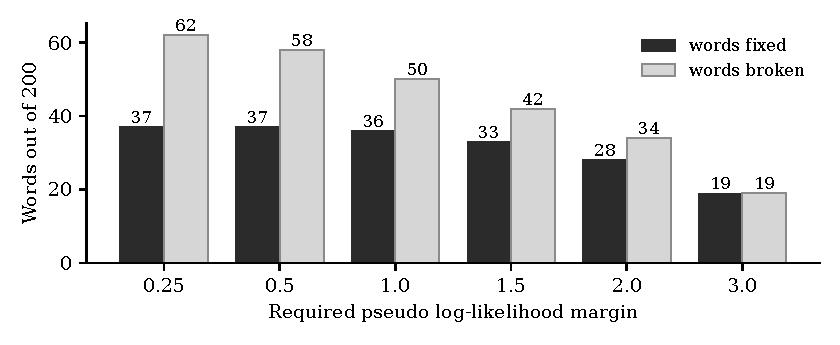
\includegraphics[width=0.92\linewidth]{figures/corrector.pdf}
\caption{Words fixed and broken by language model reranking on the 200-word
development split, at each required margin.}
\label{fig:corr}
\end{figure}

Two things limit it. The candidate set is small: of the 175 development words
that EasyOCR got wrong, the correct word was among the candidates for 48. And
I think a word in isolation gives the language model nothing to go on except
how common the word is. Several members of a confusion set are often real
words, and the model prefers the frequent one. With sentence context this
might work. On single words it does not, and the corrector ships switched off.

The first run of this experiment had a defect. A letter that belongs to two
families was only swapped within one, so a misread \ar{ن} could never be
turned back into \ar{ت}. That run fixed 20 words and broke 63 at the smallest
margin. The numbers above come from the corrected generator, and both result
files are in the repository.

A correction stage should be reported as two counts, fixes and breaks. A net
change in error rate does not show how many words the stage made worse.

\subsection{Layout model}

A wrapper for LayoutLMv3 \cite{layoutlmv3} is included. I ran it once by hand
and it returned embeddings of the expected shape. I have no labeled Arabic
documents with field annotations, so I cannot score it and make no claim
about it. Its published weights are licensed for non-commercial use only.

\section{Limitations}

The evaluation rests on one set of 2,000 small synthetic printed words whose
source I can no longer inspect. Nothing here shows how the system behaves on
scanned documents, photographs, handwriting, or text lines. The references
span only 7 to 10 characters.

Only one prompt, in Arabic, was tried. The rate of refusals and prompt echoes
may depend on it, and a different prompt could change the balance between the
engines. The degeneration flag is written around how this one model
misbehaves with this one prompt, and Section~\ref{sec:ablation} shows how
much rides on its limits. The confidence threshold was tuned on 200 words and
would need retuning for another model.

The normalization assumes Modern Standard Arabic. The arbitration numbers
come from replaying the rule over stored outputs. All timing is from one
laptop. The page mode was tried on a single image, and the visual-order repair
changed none of the stored word outputs, so its benefit is unmeasured.

\section{Availability}

The code is at \url{https://github.com/moelhaj996/mo-ocr-v3} under the Apache
License 2.0. The repository contains the run files behind the tables, the
split manifest with file hashes, a script that computes the remaining numbers
in this report from those run files, and the script that draws the figures.
The images are not redistributed, for the reasons in Section~\ref{sec:data}.
The reproduction script needs them, so for now it documents the procedure,
and the numbers can be checked by rescoring the published run files. Model
weights are downloaded at run time under their own licenses.

\section{Conclusion}

Qwen2-VL-2B and EasyOCR make different mistakes on these Arabic words, and two
cheap tests on the language model's own output choose between them well
enough to beat both. The gain over EasyOCR is a quarter of the error rate
with the flag as reported and a tenth with the flag as first written.

The obvious next step is better data. The experiment should be repeated on a
corpus with clear provenance and a license that allows redistribution, and
extended to text lines and handwriting, where the balance between the two
engines may be quite different. A flag that does not depend on a hand-set
length would remove the sensitivity found here. Fine-tuning TrOCR on matching
data would show whether a trained recognizer makes the routing unnecessary.

\section*{Use of AI tools}

I used an AI coding assistant (Claude, Anthropic) to develop the software, to
run the reviews described in Section~\ref{sec:audit}, and to draft and edit
this text. I reviewed the code, the results and the text, and I am responsible
for the content.

\begin{thebibliography}{99}
\small

\bibitem{qwen2vl}
P.~Wang, S.~Bai, S.~Tan, S.~Wang, Z.~Fan, J.~Bai, K.~Chen, X.~Liu, J.~Wang,
W.~Ge, Y.~Fan, K.~Dang, M.~Du, X.~Ren, R.~Men, D.~Liu, C.~Zhou, J.~Zhou, and
J.~Lin. Qwen2-VL: Enhancing vision-language model's perception of the world at
any resolution. arXiv:2409.12191, 2024.

\bibitem{easyocr}
JaidedAI. EasyOCR: Ready-to-use OCR with 80+ supported languages. Software,
version 1.7.2, 2024. \url{https://github.com/JaidedAI/EasyOCR}.

\bibitem{rover}
J.~G. Fiscus. A post-processing system to yield reduced word error rates:
Recognizer output voting error reduction (ROVER). In \emph{IEEE Workshop on
Automatic Speech Recognition and Understanding}, pages 347--354, 1997.

\bibitem{craft}
Y.~Baek, B.~Lee, D.~Han, S.~Yun, and H.~Lee. Character region awareness for
text detection. In \emph{IEEE/CVF Conference on Computer Vision and Pattern
Recognition}, pages 9365--9374, 2019.

\bibitem{crnn}
B.~Shi, X.~Bai, and C.~Yao. An end-to-end trainable neural network for
image-based sequence recognition and its application to scene text
recognition. \emph{IEEE Transactions on Pattern Analysis and Machine
Intelligence}, 39(11):2298--2304, 2017.

\bibitem{trocr}
M.~Li, T.~Lv, J.~Chen, L.~Cui, Y.~Lu, D.~Florencio, C.~Zhang, Z.~Li, and
F.~Wei. TrOCR: Transformer-based optical character recognition with
pre-trained models. \emph{Proceedings of the AAAI Conference on Artificial
Intelligence}, 37(11):13094--13102, 2023.

\bibitem{mlmscoring}
J.~Salazar, D.~Liang, T.~Q. Nguyen, and K.~Kirchhoff. Masked language model
scoring. In \emph{Annual Meeting of the Association for Computational
Linguistics}, pages 2699--2712, 2020.

\bibitem{camelbert}
G.~Inoue, B.~Alhafni, N.~Baimukan, H.~Bouamor, and N.~Habash. The interplay of
variant, size, and task type in Arabic pre-trained language models. In
\emph{Sixth Arabic Natural Language Processing Workshop}, pages 92--104, 2021.

\bibitem{layoutlmv3}
Y.~Huang, T.~Lv, L.~Cui, Y.~Lu, and F.~Wei. LayoutLMv3: Pre-training for
document AI with unified text and image masking. In \emph{ACM International
Conference on Multimedia}, pages 4083--4091, 2022.

\bibitem{apti}
F.~Slimane, R.~Ingold, S.~Kanoun, A.~M. Alimi, and J.~Hennebert. A new Arabic
printed text image database and evaluation protocols. In \emph{International
Conference on Document Analysis and Recognition}, pages 946--950, 2009.

\bibitem{khatt}
S.~A. Mahmoud, I.~Ahmad, W.~G. Al-Khatib, M.~Alshayeb, M.~T. Parvez,
V.~M\"argner, and G.~A. Fink. KHATT: An open Arabic offline handwritten text
database. \emph{Pattern Recognition}, 47(3):1096--1112, 2014.

\bibitem{efron}
B.~Efron and R.~J. Tibshirani. \emph{An Introduction to the Bootstrap}.
Chapman \& Hall, 1993.

\bibitem{koehn}
P.~Koehn. Statistical significance tests for machine translation evaluation.
In \emph{Conference on Empirical Methods in Natural Language Processing},
pages 388--395, 2004.

\bibitem{uax15}
The Unicode Consortium. Unicode Standard Annex \#15: Unicode normalization
forms. \url{https://www.unicode.org/reports/tr15/}, read September 2026.

\bibitem{habash}
N.~Y. Habash. \emph{Introduction to Arabic Natural Language Processing}.
Synthesis Lectures on Human Language Technologies. Morgan \& Claypool, 2010.

\bibitem{levenshtein}
V.~I. Levenshtein. Binary codes capable of correcting deletions, insertions,
and reversals. \emph{Soviet Physics Doklady}, 10(8):707--710, 1966.

\end{thebibliography}

\end{document}
